\newpage
\section{Installation et utilisation}

Le programme, qui est programmé en Java, est assez simple d'utilisation. En effet, ce dernier ne requiert aucune installation particulière, mais plutot une mise en place de certains éléments. 

\subsection{Installation}

\subsection{Utilisation}

Lors du lancement du programme, l'utilisateur se verra demandé ce qu'il souhaite faire : 
\begin{itemize}
\item Lire un code-barre à partir d'un fichier image
\item Générer un code-barre à partir d'un texte qu'il devra fournir
\end{itemize}

Via la commande, l'utilisateur choisira donc l'action qu'il souhaite effectuer (cfr figure 1). Ensuite, l'utilisateur sera guidé à travers les différentes étapes pour la lecture et la génération de CB2D. L'utilisateur n'aura aucun problème pour utiliser le programme car l'interface de ce dernier est facile à comprendre et très intuitive. 

\begin{figure}[!h]
	\centering
	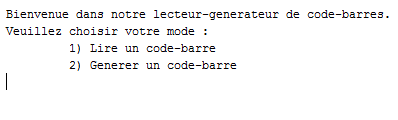
\includegraphics[width=0.7\textwidth]{images/choixMode.png}
	\caption{Choix du mode d'utilisation}  
	\label{Choix du mode d'utilisation}
\end{figure}



\subsubsection{Lecture}

Si l'utilisateur choisit de lire un code-barre, il lui sera demandé de spécifié le chemin d'accès au fichier image qui contient le CB2D. Ensuite, l'utilisateur n'aura plus qu'à attendre que le programme décode le CB2D et qu'il en extraie les informations contenues.

Ensuite, les informations seront présentées à l'utilisateur.

\subsubsection{Génération}

Si en revanche l'utilisateur choisit de générer un code-barre, il devra alors fournir les informations à stocker, sous forme de texte, au programme. Le programme va ensuite encoder les informations et les transformer en CB2D, qui sera ensuite imprimé et sauvegardé dans un fichier image.